\documentclass[border=15pt]{standalone}
\usepackage{tikz,amsmath}
\usetikzlibrary{arrows.meta}

% ========== 配色方案（Inception 调色板体系） ==========
% 顶部输入特征图（自然绿）
\definecolor{inFill}{RGB}{183,224,177}
\definecolor{inLine}{RGB}{32,102,32}

% 分支 1 与后置 1x1 Conv：浅蓝紫内底，深蓝紫描边
\definecolor{hidFill}{RGB}{199,203,243}
\definecolor{hidLine}{RGB}{52,58,143}

% 分支 2：3x3 Conv, rate=1（浅暖橙内底，深暖橙描边）
\definecolor{orFill}{RGB}{250,224,180}
\definecolor{orLine}{RGB}{190,110,20}

% 分支 3：3x3 Conv, rate=2（浅珊瑚红内底，深红描边）
\definecolor{outFill}{RGB}{243,199,199}
\definecolor{outLine}{RGB}{143,52,52}

% 分支 4：3x3 Conv, rate=3（浅纯蓝内底，深蓝描边）
\definecolor{blFill}{RGB}{214,228,250}
\definecolor{blLine}{RGB}{60,90,170}

% 分支 5：Image Pooling（雅致香芋紫）
\definecolor{gapFill}{RGB}{236,220,248}
\definecolor{gapLine}{RGB}{125,50,150}

% 底部最终输出特征图（沉稳翠绿）
\definecolor{postFill}{RGB}{202,232,216}
\definecolor{postLine}{RGB}{28,110,75}

\begin{document}
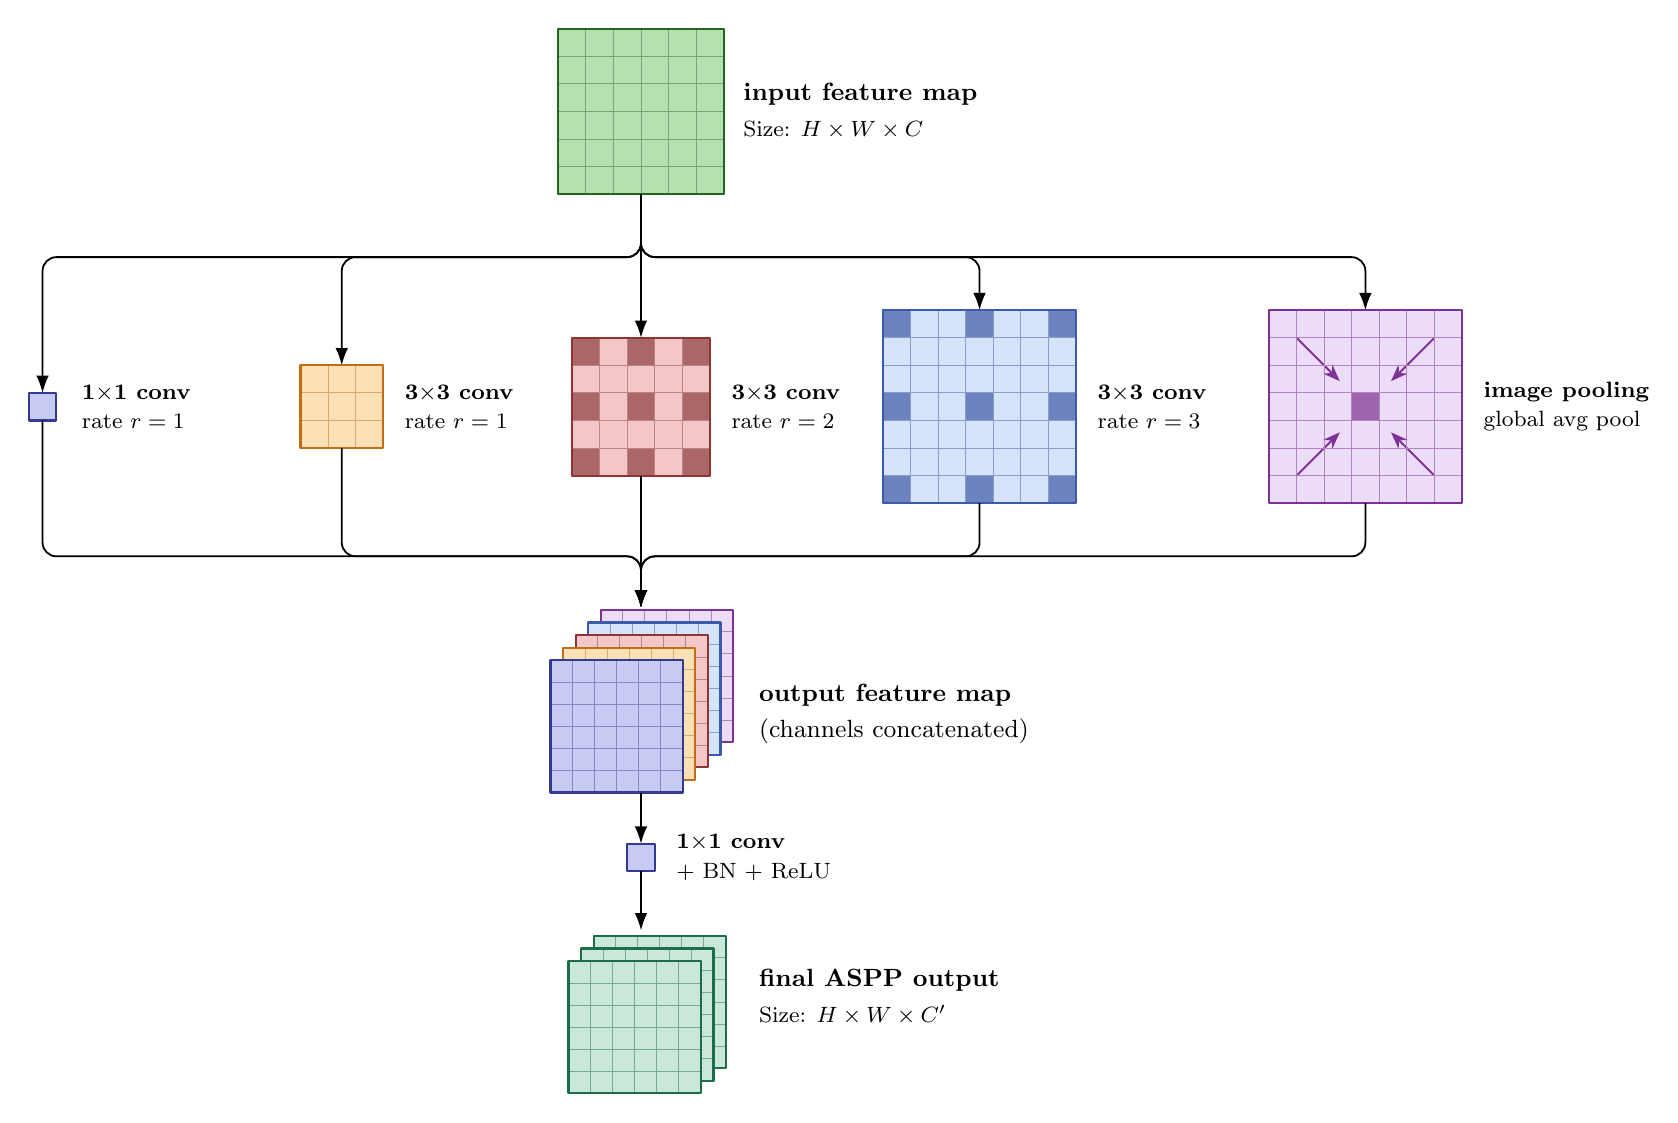
\begin{tikzpicture}[
    font=\small, line join=round,
    every node/.style={inner sep=0pt, outer sep=0pt},
    >={Latex[length=2.2mm, width=1.6mm]},
    arr/.style={->, line width=.65pt, rounded corners=5pt}
  ]

  % ========== 通用网格方块宏 ==========
  \newcommand{\gridbox}[5]{%
    \fill[#5Fill] (#1,#2) rectangle (#1+#3*#4, #2+#3*#4);
    \draw[step=#4, #5Line!60, line width=.35pt, shift={(#1,#2)}] (0,0) grid (#3*#4, #3*#4);
    \draw[#5Line, thick] (#1,#2) rectangle (#1+#3*#4, #2+#3*#4);
  }

  % 1. 顶部：输入特征图 (Input Feature Map)
  \gridbox{-1.05}{6.3}{6}{.35}{in}
  \node[anchor=west, align=left] at (1.3, 7.35) {
    \textbf{input feature map}\\[2pt]
    {\footnotesize Size: $H \times W \times C$}
  };

  % 2. 输入 -> 5 分支连线 (分流 Bus y = 5.5)
  % 分支水平中心 X = -7.6, -3.8, 0.0, 4.3, 9.2
  \draw[arr] (0, 6.3) -- (0, 5.5) -- (-7.6, 5.5) -- (-7.6, 3.775);
  \draw[arr] (0, 6.3) -- (0, 5.5) -- (-3.8, 5.5) -- (-3.8, 4.125);
  \draw[arr] (0, 6.3) -- (0, 4.475);
  \draw[arr] (0, 6.3) -- (0, 5.5) -- (4.3, 5.5)  -- (4.3, 4.825);
  \draw[arr] (0, 6.3) -- (0, 5.5) -- (9.2, 5.5)  -- (9.2, 4.825);

  % 3. 五大核心分支（统一垂直居中 y = 3.6，文字全部位于右侧）
  % ---------- 分支 1：1x1 Conv ----------
  \gridbox{-7.775}{3.425}{1}{.35}{hid}
  \node[anchor=west, align=left, font=\footnotesize] at (-7.1, 3.6) {
    \textbf{1$\times$1 conv}\\[1pt]
    rate $r = 1$
  };

  % ---------- 分支 2：3x3 Conv ----------
  \gridbox{-4.325}{3.075}{3}{.35}{or}
  \node[anchor=west, align=left, font=\footnotesize] at (-3.0, 3.6) {
    \textbf{3$\times$3 conv}\\[1pt]
    rate $r = 1$
  };

  % ---------- 分支 3：3x3 空洞卷积 (5x5 跨度网格，步长为 2) ----------
  \begin{scope}[shift={(-0.875, 2.725)}]
    \fill[outFill] (0, 0) rectangle (1.75, 1.75);
    \foreach \r in {0,2,4} {
      \foreach \c in {0,2,4} {
        \fill[outLine!75] (\c*0.35, \r*0.35) rectangle ++(0.35, 0.35);
      }
    }
    \draw[step=0.35, outLine!60, line width=.35pt] (0, 0) grid (1.75, 1.75);
    \draw[outLine, thick] (0, 0) rectangle (1.75, 1.75);
  \end{scope}
  \node[anchor=west, align=left, font=\footnotesize] at (1.15, 3.6) {
    \textbf{3$\times$3 conv}\\[1pt]
    rate $r = 2$
  };

  % ---------- 分支 4：3x3 空洞卷积 (7x7 跨度网格，步长为 3) ----------
  \begin{scope}[shift={(3.075, 2.375)}]
    \fill[blFill] (0, 0) rectangle (2.45, 2.45);
    \foreach \r in {0,3,6} {
      \foreach \c in {0,3,6} {
        \fill[blLine!75] (\c*0.35, \r*0.35) rectangle ++(0.35, 0.35);
      }
    }
    \draw[step=0.35, blLine!60, line width=.35pt] (0, 0) grid (2.45, 2.45);
    \draw[blLine, thick] (0, 0) rectangle (2.45, 2.45);
  \end{scope}
  \node[anchor=west, align=left, font=\footnotesize] at (5.8, 3.6) {
    \textbf{3$\times$3 conv}\\[1pt]
    rate $r = 3$
  };

  % ---------- 分支 5：Image Pooling (全局平均池化，雅致香芋紫) ----------
  \begin{scope}[shift={(7.975, 2.375)}]
    \fill[gapFill] (0, 0) rectangle (2.45, 2.45);
    % 向中心汇聚的指示箭头
    \draw[->, >=Stealth, gapLine, line width=0.7pt] (0.35, 2.10) -- (0.90, 1.55);
    \draw[->, >=Stealth, gapLine, line width=0.7pt] (2.10, 2.10) -- (1.55, 1.55);
    \draw[->, >=Stealth, gapLine, line width=0.7pt] (0.35, 0.35) -- (0.90, 0.90);
    \draw[->, >=Stealth, gapLine, line width=0.7pt] (2.10, 0.35) -- (1.55, 0.90);
    % 中心池化像素
    \fill[gapLine!75] (3*0.35, 3*0.35) rectangle ++(0.35, 0.35);
    \draw[step=0.35, gapLine!60, line width=.35pt] (0, 0) grid (2.45, 2.45);
    \draw[gapLine, thick] (0, 0) rectangle (2.45, 2.45);
  \end{scope}
  \node[anchor=west, align=left, font=\footnotesize] at (10.7, 3.6) {
    \textbf{image pooling}\\[1pt]
    global avg pool
  };

  % 4. 五分支 -> 汇合 -> 通道拼接堆 (Merge Bus y = 1.7)
  \draw[arr] (-7.6, 3.425) -- (-7.6, 1.7) -- (0, 1.7) -- (0, 1.05);
  \draw[arr] (-3.8, 3.075) -- (-3.8, 1.7) -- (0, 1.7) -- (0, 1.05);
  \draw[arr] (0, 2.725)    -- (0, 1.05);
  \draw[arr] (4.3, 2.375)  -- (4.3, 1.7)  -- (0, 1.7) -- (0, 1.05);
  \draw[arr] (9.2, 2.375)  -- (9.2, 1.7)  -- (0, 1.7) -- (0, 1.05);

  % 5. 底部：5 分支通道维拼接堆叠 (Depth Concatenation)
  \gridbox{-0.51}{-0.66}{6}{.28}{gap}  % Image Pooling
  \gridbox{-0.67}{-0.82}{6}{.28}{bl}   % Rate 3
  \gridbox{-0.83}{-0.98}{6}{.28}{out}  % Rate 2
  \gridbox{-0.99}{-1.14}{6}{.28}{or}   % Rate 1
  \gridbox{-1.15}{-1.30}{6}{.28}{hid}  % 1x1 Conv

  \node[anchor=west, align=left] at (1.5, -0.3) {
    \textbf{output feature map}\\[2pt]
    (channels concatenated)
  };

  % 6. 拼接后 -> 1x1 卷积图标（文字同样放于右侧）
  \draw[arr] (0, -1.30) -- (0, -1.95);

  \gridbox{-0.175}{-2.30}{1}{.35}{hid}
  \node[anchor=west, align=left, font=\footnotesize] at (0.45, -2.125) {
    \textbf{1$\times$1 conv}\\[1pt]
    $+$ BN $+$ ReLU
  };

  % 7. 降维后 -> 最终输出特征图 (Final ASPP Output)
  \draw[arr] (0, -2.30) -- (0, -3.05);

  \gridbox{-0.60}{-4.80}{6}{.28}{post}
  \gridbox{-0.76}{-4.96}{6}{.28}{post}
  \gridbox{-0.92}{-5.12}{6}{.28}{post}

  \node[anchor=west, align=left] at (1.5, -3.9) {
    \textbf{final ASPP output}\\[2pt]
    {\footnotesize Size: $H \times W \times C'$}
  };

\end{tikzpicture}
\end{document}